\documentclass{standalone}
\usepackage{pgf}
\usepackage{amsmath}
\usepackage{tikz}
\usetikzlibrary{shapes,arrows}
\usetikzlibrary{positioning}
\begin{document}
   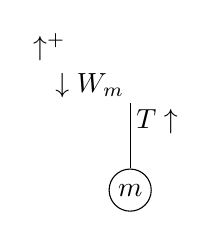
\begin{tikzpicture}[
    node distance = 0mm,
every node/.style = {inner sep=2pt}]
\coordinate                     (a)  at (0,0);
\coordinate[below=11mm of a]    (b);
\node[circle,draw,minimum size=3mm, 
      at=(b)]            (c)    {$m$};
    \draw (a) -- (c);
\node[below right=of a]         {$T\uparrow$};
\node[above left =of a]  (d)    {$\downarrow W_m$};
\node[above=of d.north west]    {$\uparrow^+$};
    \end{tikzpicture}
\end{document}
